\documentclass[10pt,a4paper]{article}
\usepackage[margin=.75in]{geometry}\usepackage[T1]{fontenc}
\usepackage{lmodern,microtype,booktabs,graphicx,xcolor,hyperref}
\hypersetup{hidelinks}\setlength{\parindent}{0pt}\setlength{\parskip}{6pt}\emergencystretch=2em
\title{IDM-Viz: Future-Harm Forecast Under an Unseen Synthetic Law}
\author{Ahmed Bilal (23I-2581) \and Umar Behram (23I-2604)}\date{16 November 2026}
\begin{document}\maketitle
\begin{abstract}
We evaluated the existing five-batch harm forecaster on a conditional-randomization synthetic mechanism withheld from forecaster training, with its onset balanced across four batches on 30 held-out seeds. The best monitor-based predictors outperform the development-prevalence baseline in Brier score, but a time-only model remains strong, released-label history adds no clear Brier benefit in this follow-up, and the result remains limited to one manually designed synthetic law.
\end{abstract}
\section{Why a second held-out run was needed}
An initial run placed the new mechanism's onset at the same one-based row 4001 used by several training conditions. The time-only predictor then reached ROC AUC 0.998, revealing that the fixed timeline made the future target almost predictable without monitoring evidence. We retain the pilot output and do not interpret it as convincing transfer. This follow-up balances the onset across batches 5, 9, 13 and 17 across evaluation seeds before scoring.
\section{Locked protocol}
The new label law uses $p_{new}=(1-0.70)p_{base}+0.70\times0.5$ after the assigned onset; the X generation is identical before and after onset. The three forecasters are retrained deterministically only on the saved original 30 development seeds and C0-C6 data, with the unchanged feature lists, StandardScaler and LogisticRegression(C=1). Evaluation uses 30 disjoint seeds, all four balanced onset positions, 19 origins, the target that next-five-batch mean accuracy is more than 0.05 below the stream's historical reference, and delays 0/5/20. A monitoring label from batch $b$ and delay $d$ is available only if $b+d<t$ for the forecast batch $t$; same-clock labels are added afterward. Seed and condition IDs are not predictors. Prevalence, last released harm and current concern are comparators, not fitted models.
\section{Results}
\begin{table}[ht]\centering\small\begin{tabular}{lrrrr}\toprule Predictor & ROC AUC & AP & Brier & Log loss \\\midrule
Time only & 0.875 & 0.942 & 0.238 & 0.669 \\
Unlabeled monitor & 0.864 & 0.940 & 0.188 & 0.561 \\
Released-label model & 0.830 & 0.922 & 0.194 & 0.574 \\
Development prevalence & 0.500 & 0.693 & 0.290 & 0.774 \\
Last released harm & 0.636 & 0.794 & 0.333 & 4.183 \\
Current concern & 0.465 & 0.695 & 0.660 & 4.022 \\
\bottomrule\end{tabular}\caption{30 held-out seeds, four onset positions, three delays and 19 forecast origins (1,710 rows per predictor). Target prevalence was 0.693. AP should be read against that prevalence. Current concern and last-harm values are raw heuristic scores, not calibrated future probabilities.} \end{table}
\begin{figure}[ht]\centering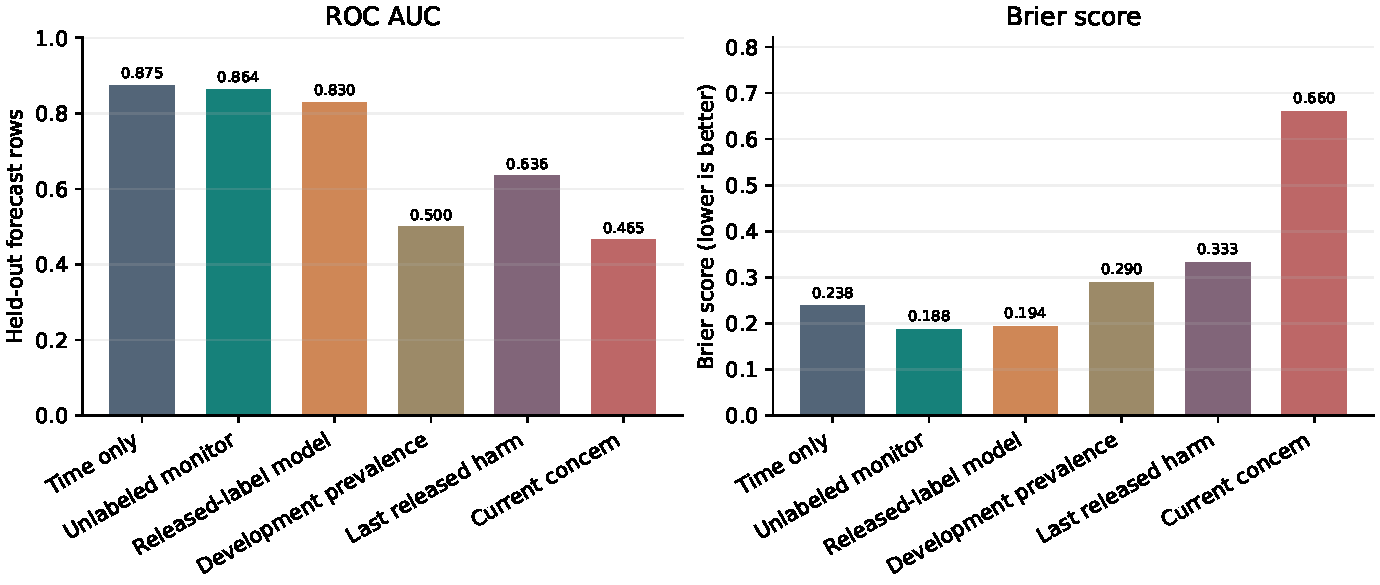
\includegraphics[width=.97\linewidth]{unseen_family_metrics.pdf}\caption{Held-out performance for the balanced-onset conditional-randomization law.}
\end{figure}
\subsection{Paired seed-level Brier differences}
The contrast is first predictor minus second; positive values favor the second predictor.
\begin{table}[ht]\centering\small\begin{tabular}{lrr}\toprule Contrast & Mean difference & 95\% seed-bootstrap interval \\\midrule
time only minus unlabeled monitor Brier & +0.0506 & [+0.0408, +0.0619] \\
unlabeled monitor minus full released Brier & -0.0067 & [-0.0229, +0.0086] \\
time only minus full released Brier & +0.0439 & [+0.0218, +0.0665] \\
full released minus development prevalence Brier & -0.0956 & [-0.1081, -0.0824] \\
\bottomrule\end{tabular}\caption{Two thousand paired bootstrap replicates resample 30 held-out seeds as clusters and retain each seed's delays and forecast origins.} \end{table}
Time-only Brier was 0.238 and unlabeled-monitor Brier 0.188; the time-only-minus-unlabeled contrast was +0.0506 [0.0408, 0.0619]. The released-label model had Brier 0.194; the unlabeled-minus-released contrast was -0.0067 [-0.0229, 0.0086], which does not establish a released-label benefit. The development-prevalence Brier was 0.290. These are seed-conditional synthetic results, not population guarantees.
\section{Interpretation and limitations}
Balancing onset weakens but does not eliminate temporal predictability (time-only AUC 0.875). Monitor evidence improves probability error versus time alone and the prevalence constant in this designed law, while adding released labels does not show a clear Brier gain over unlabeled features under this schedule. The initial aligned-onset pilot is a useful warning about temporal confounding, not evidence to hide. The new law is manually designed and closely related to the baseline logistic construction; four onset values do not represent arbitrary drift families. This is not external-domain validation, causal identification, analyst-benefit evidence, a calibrated risk certificate, or proof of broad generalization.
\section{Reproduction}
\begin{verbatim}
python scripts/run_future_harm_unseen_family.py --onset-policy balanced_onsets --out RUN
python scripts/evaluate_future_harm_unseen_family.py --run RUN
python scripts/report_future_harm_unseen_family.py --run RUN --out REPORT
\end{verbatim}
\end{document}
